% Options for packages loaded elsewhere
\PassOptionsToPackage{unicode}{hyperref}
\PassOptionsToPackage{hyphens}{url}
\PassOptionsToPackage{dvipsnames,svgnames,x11names}{xcolor}
%
\documentclass[
  11pt,
]{article}
\usepackage{amsmath,amssymb}
\usepackage{iftex}
\ifPDFTeX
  \usepackage[T1]{fontenc}
  \usepackage[utf8]{inputenc}
  \usepackage{textcomp} % provide euro and other symbols
\else % if luatex or xetex
  \usepackage{unicode-math} % this also loads fontspec
  \defaultfontfeatures{Scale=MatchLowercase}
  \defaultfontfeatures[\rmfamily]{Ligatures=TeX,Scale=1}
\fi
\usepackage{lmodern}
\ifPDFTeX\else
  % xetex/luatex font selection
\fi
% Use upquote if available, for straight quotes in verbatim environments
\IfFileExists{upquote.sty}{\usepackage{upquote}}{}
\IfFileExists{microtype.sty}{% use microtype if available
  \usepackage[]{microtype}
  \UseMicrotypeSet[protrusion]{basicmath} % disable protrusion for tt fonts
}{}
\makeatletter
\@ifundefined{KOMAClassName}{% if non-KOMA class
  \IfFileExists{parskip.sty}{%
    \usepackage{parskip}
  }{% else
    \setlength{\parindent}{0pt}
    \setlength{\parskip}{6pt plus 2pt minus 1pt}}
}{% if KOMA class
  \KOMAoptions{parskip=half}}
\makeatother
\usepackage{xcolor}
\usepackage[margin=1in]{geometry}
\usepackage{listings}
\newcommand{\passthrough}[1]{#1}
\lstset{defaultdialect=[5.3]Lua}
\lstset{defaultdialect=[x86masm]Assembler}
\usepackage{longtable,booktabs,array}
\usepackage{calc} % for calculating minipage widths
% Correct order of tables after \paragraph or \subparagraph
\usepackage{etoolbox}
\makeatletter
\patchcmd\longtable{\par}{\if@noskipsec\mbox{}\fi\par}{}{}
\makeatother
% Allow footnotes in longtable head/foot
\IfFileExists{footnotehyper.sty}{\usepackage{footnotehyper}}{\usepackage{footnote}}
\makesavenoteenv{longtable}
\usepackage{graphicx}
\makeatletter
\def\maxwidth{\ifdim\Gin@nat@width>\linewidth\linewidth\else\Gin@nat@width\fi}
\def\maxheight{\ifdim\Gin@nat@height>\textheight\textheight\else\Gin@nat@height\fi}
\makeatother
% Scale images if necessary, so that they will not overflow the page
% margins by default, and it is still possible to overwrite the defaults
% using explicit options in \includegraphics[width, height, ...]{}
\setkeys{Gin}{width=\maxwidth,height=\maxheight,keepaspectratio}
% Set default figure placement to htbp
\makeatletter
\def\fps@figure{htbp}
\makeatother
\setlength{\emergencystretch}{3em} % prevent overfull lines
\providecommand{\tightlist}{%
  \setlength{\itemsep}{0pt}\setlength{\parskip}{0pt}}
\setcounter{secnumdepth}{5}
\definecolor{codegreen}{rgb}{0,0.6,0}
\definecolor{codegray}{rgb}{0.5,0.5,0.5}
\definecolor{codepurple}{rgb}{0.58,0,0.82}
\definecolor{backcolour}{rgb}{0.95,0.95,0.92}

\lstdefinestyle{mystyle}{
    backgroundcolor=\color{backcolour},
    commentstyle=\color{codegreen},
    keywordstyle=\color{magenta},
    numberstyle=\tiny\color{codegray},
    stringstyle=\color{codepurple},
    basicstyle=\ttfamily\footnotesize,
    breakatwhitespace=true,
    breaklines=true,
    captionpos=b,
    keepspaces=true,
    numbers=left,
    numbersep=5pt,
    showspaces=false,
    showstringspaces=false,
    showtabs=false,
    tabsize=2,
    morekeywords={function, if, else, for, while, repeat, in, next, break, TRUE, FALSE, NULL, NA, NaN, Inf}, % Additional keywords
    escapeinside={(*@}{@*)}
}

\lstset{
  breaklines=true,
  language=R,
  style=mystyle
}
\usepackage{physics}
\usepackage{bm}
\usepackage{booktabs}
\usepackage{longtable}
\usepackage{array}
\usepackage{multirow}
\usepackage{wrapfig}
\usepackage{float}
\usepackage{colortbl}
\usepackage{pdflscape}
\usepackage{tabu}
\usepackage{threeparttable}
\usepackage{threeparttablex}
\usepackage[normalem]{ulem}
\usepackage{makecell}
\usepackage{xcolor}
\ifLuaTeX
  \usepackage{selnolig}  % disable illegal ligatures
\fi
\usepackage{bookmark}
\IfFileExists{xurl.sty}{\usepackage{xurl}}{} % add URL line breaks if available
\urlstyle{same}
\hypersetup{
  pdftitle={Depression and Associated Risk Factors: NHANES Data Analysis MATH70076-Assessment 2},
  pdfauthor={02051768},
  colorlinks=true,
  linkcolor={blue},
  filecolor={Maroon},
  citecolor={Blue},
  urlcolor={Blue},
  pdfcreator={LaTeX via pandoc}}

\title{Depression and Associated Risk Factors: NHANES Data Analysis MATH70076-Assessment 2}
\author{02051768}
\date{2025-05-11}

\begin{document}
\maketitle

{
\hypersetup{linkcolor=}
\setcounter{tocdepth}{2}
\tableofcontents
}
\newpage

\section{Background}\label{background}

The aim of this report is to assess the relationship between depression and a range of influencing factors. We used data from the DEMO, DPQ, ALQ, SMQ, PAD, DIQ, and MCQ modules in NHANES, covering the survey years 2015--2018 and 2021--2023. The pandemic period (2019--2020) was deliberately excluded, as population-level mental health during that time may have been atypical due to public health policies and societal disruptions

\section{Data Downloading \& Cleaning}\label{data-downloading-cleaning}

The data was downloaded using the \passthrough{\lstinline!nhanesA!} package. It can also be accessed from the official website \href{https://wwwn.cdc.gov/nchs/nhanes/}{NHANES}. Data files from each selected year were merged into a single dataset (\passthrough{\lstinline!combined\_data!}), retaining only variables that were consistently available across all years.

To calculate the PHQ-9 total score (\passthrough{\lstinline!PHQ\_total!}), we processed the DPQ section of the NHANES dataset, which records participants' responses of nine items assessing depressive symptoms. Each item was recoded numerically according to the standard PHQ-9 scoring scheme: ``Not at all'' = 0, ``Several days'' = 1, ``More than half the days'' = 2, and ``Nearly every day'' = 3. Responses coded as ``Refused'' or ``Don't know'' were treated as missing values. The \passthrough{\lstinline!PHQ\_total!} was then computed by summing the numeric values of the first nine items. This \passthrough{\lstinline!PHQ\_total!} ranging from 0 to 27,presenting depression severity (higher scores representing more severe depressive symptoms). Then all data with missing value in \passthrough{\lstinline!PHQ\_total!} were removed as \passthrough{\lstinline!PHQ\_total!} is the key of the study.

For the rest of the potentially correlated variables, we simply performed basic cleaning and converted them into a standard format. All categorical variables were converted to factors, and responses labeled ``Refused'' or ``Don't Know'' were recoded as missing values. For numerical variables, we applied as.numeric to ensure proper data types. After reviewing the data summary, we selected a subset of variables for further analysis based on their relevance, type, value distributions, and proportion of missing data. The final dataset includes: \passthrough{\lstinline!gender!}, \passthrough{\lstinline!race!}, (\passthrough{\lstinline!edu!}), \passthrough{\lstinline!birth\_country!}, \passthrough{\lstinline!military!}, \passthrough{\lstinline!heavy\_drinker!}, \passthrough{\lstinline!ever\_smoked!}, \passthrough{\lstinline!diabetes!},\passthrough{\lstinline!has\_asthma!}, \passthrough{\lstinline!hay\_fever!}, \passthrough{\lstinline!has\_liver!}, \passthrough{\lstinline!has\_cancer!}, \passthrough{\lstinline!PHQ\_total!}, \passthrough{\lstinline!age!}, household size (\passthrough{\lstinline!hh\_size!}), \passthrough{\lstinline!drinks\_per\_day!}, \passthrough{\lstinline!sedentary\_minutes!}, and \passthrough{\lstinline!poverty\_ratio!}. We also filtered out rows with missing values in variables that had low rates of missingness (specifically: \passthrough{\lstinline!edu!}, \passthrough{\lstinline!birth\_country!}, \passthrough{\lstinline!military!}, \passthrough{\lstinline!ever\_smoked!}, \passthrough{\lstinline!PHQ\_total!}, \passthrough{\lstinline!has\_asthma!}, \passthrough{\lstinline!sedentary\_minutes!}, and \passthrough{\lstinline!has\_liver!}). This helped us retain more data points and ensure the completeness of the selected variables. Now, we have the final data (\passthrough{\lstinline!analysis\_data!}) for analysis.

\section{Exploratory data analysis}\label{exploratory-data-analysis}

After basic preprocessing and reviewing the summary of \passthrough{\lstinline!analysis\_data!}, the variables \passthrough{\lstinline!drinks\_per\_day!} and \passthrough{\lstinline!hay\_fever!} were dropped due to their relatively high missing rates. We also redefined the reference categories of categorical variables to improve interpretability for the model. To handle missing values in \passthrough{\lstinline!poverty\_ratio!}, we filled the NAs with its median after the EDA part, ensuring minimal distortion of its distribution. For the only two categorical variables with missing values (\passthrough{\lstinline!heavy\_drinker!} and \passthrough{\lstinline!diabetes!}), we kept the NA values as a separate category.The non-response is treated as potentially informative as an evasive answer may also reflect the respondent's attitude toward the question. What's more, we observed that Non-Hispanic White participants (n = 6522) take the majority of the sample, while some racial groups seems to be underrepresented. I also noticed the high concentration in higher education level so we combined the two lowest education categories into one group to simplify interpretation.

Firstly, the density plot below below shows that PHQ-9 scores are highly right-skewed, with most values concentrated near zero and a mean of 3.5. The majority of participants shows minimal depressive symptoms and the long tail presents a smaller subgroup experiencing moderate to severe symptoms.

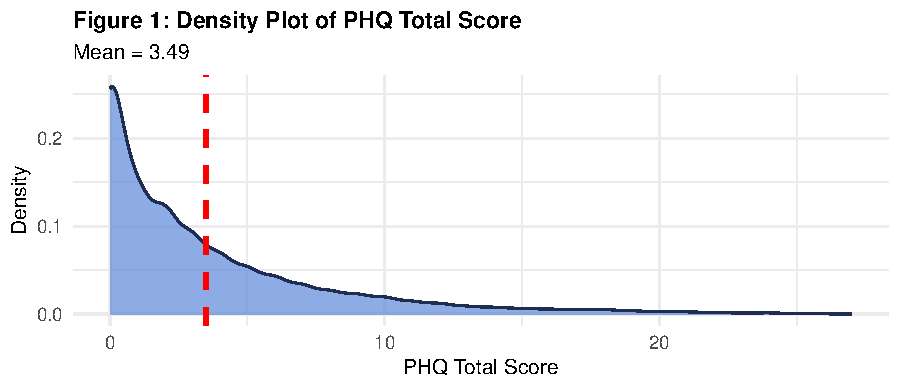
\includegraphics{report_files/figure-latex/plot_phq_density1-1.pdf}

\subsection{Categorical variables}\label{categorical-variables}

Now, let's focus on how multiple categorical variables relate to depression levels. The density plot of PHQ scores by gender (Figure 1) clearly shows that females tend to have higher average depression levels compared to males. The violin plot (Figure 2) indicates that participants with asthma generally have slightly higher PHQ-9 scores, with more values falling in the moderate-to-severe range compared to those without asthma.

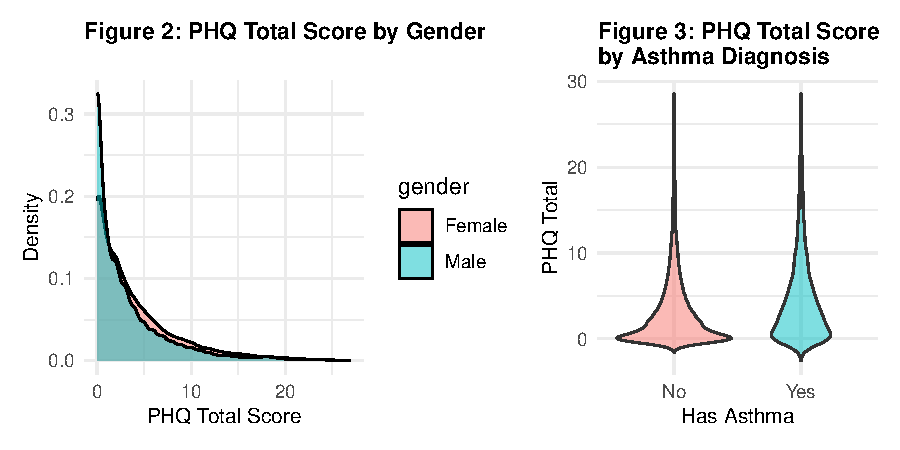
\includegraphics{report_files/figure-latex/plot_gender_Asthma-1.pdf}

According to the box plot below, heavy drinkers tend to show higher levels of depressive symptoms compared to others (Figure 4). Interestingly, there's a curious observation that resonates with a common belief in traditional Chinese medicine---that emotional disturbances are often linked to liver health. As shown in Figure 5, participants with liver conditions appear to have higher PHQ-9 scores on average.

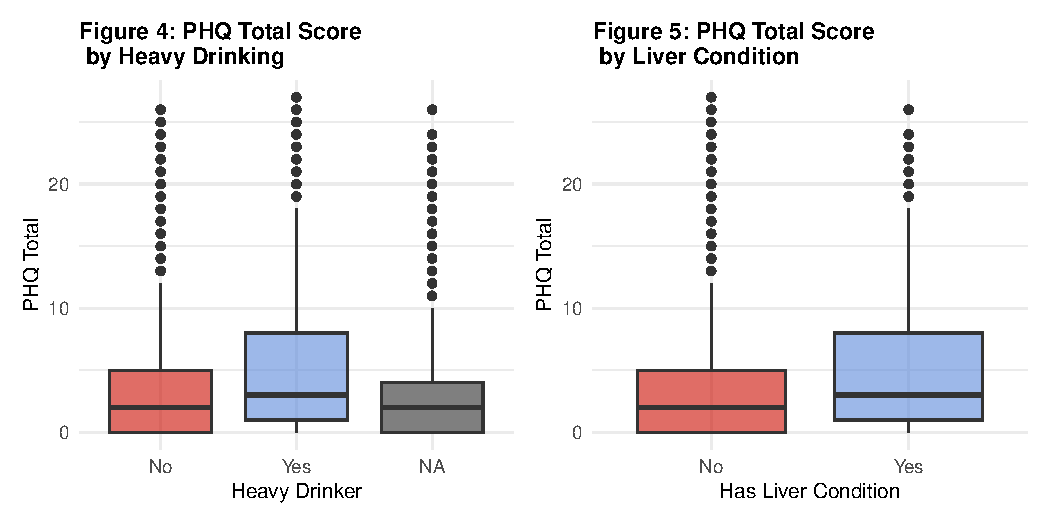
\includegraphics{report_files/figure-latex/plot_drink_liver-1.pdf}

The boxplot of PHQ total scores by race and the race distribution pie chart below are used to explore the relationship between race and depression levels. As shown in Figure 6, Non-Hispanic Asians appear to have the lowest levels of depressive symptoms on average. Interestingly, the group with the smallest population share---Other Race, Including Multi-Racial---shows relatively higher PHQ scores. This could be influenced by a range of factors such as identity-related stress, cultural marginalization, or limited access to mental health resources.

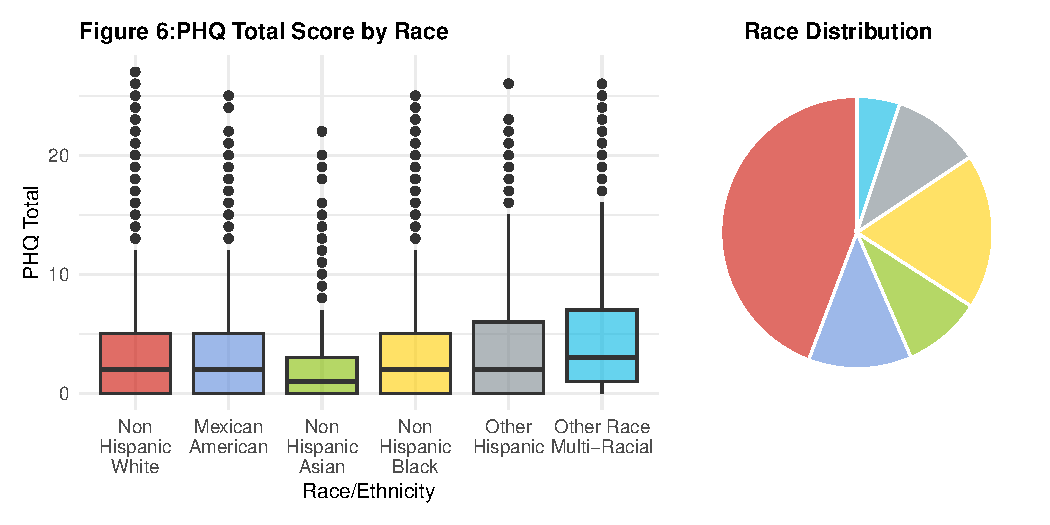
\includegraphics{report_files/figure-latex/plot_race-1.pdf}

Using the similar analysis approach, we also explored the relationship between PHQ scores and other categorical variables. We found that participants who were born in the U.S., or who have diabetes or asthma, tend to report slightly higher levels of depressive symptoms. In contrast, PHQ scores appeared to show little or no association with variables such as \passthrough{\lstinline!ever\_smoked!}, \passthrough{\lstinline!education level!}, \passthrough{\lstinline!military service!}, or \passthrough{\lstinline!cancer diagnosis!}. A summary table of the variables showing notable differences is provided below for reference. This really surprised me, as these factors are commonly believed to be associated with depression risk, such as the PTSD experiences of military and the panic of patient. Here, we do not include the corresponding plots in the main body of this report, they can be found in the accompanying R script. The table below presents the remaining correlated variables and provides some basic insight into the selected features.

\begin{table}[!h]
\centering
\caption{\label{tab:table}Summary Statistics of PHQ9 Scores}
\centering
\resizebox{\ifdim\width>\linewidth\linewidth\else\width\fi}{!}{
\begin{tabular}[t]{l|l|l|l|l|l|l}
\hline
variable & group & count & mean\_PHQ & median\_PHQ & sd\_PHQ & IQR\_PHQ\\
\hline
Has Asthma & No & 12330 & 3.25 & 2 & 4.20 & 5\\
\hline
Has Asthma & Yes & 2415 & 4.73 & 3 & 5.08 & 6\\
\hline
Diabetes & No & 12123 & 3.33 & 2 & 4.25 & 5\\
\hline
Diabetes & Yes & 2183 & 4.31 & 3 & 5.00 & 6\\
\hline
Diabetes & NA & 439 & 3.86 & 2 & 4.56 & 6\\
\hline
Birth Country & US-born & 10841 & 3.72 & 2 & 4.52 & 5\\
\hline
Birth Country & Foreign-born & 3904 & 2.87 & 1 & 3.95 & 4\\
\hline
\end{tabular}}
\end{table}

\subsection{Numerical variables}\label{numerical-variables}

We now turn to the effects of numerical variables on depression levels. In Figure 7, there appears to be an exponential relationship between sedentary time and PHQ-9 scores. The participants who report more sedentary minutes tend to have higher levels of depressive symptoms. In contrast, Figure 8 shows that participants with higher poverty ratios (indicating higher income relative to the poverty threshold) generally report lower depression scores, indicating that better socioeconomic conditions are associated with better mental health. Additionally, we observe that older participants tend to report lower levels of depressive symptoms.

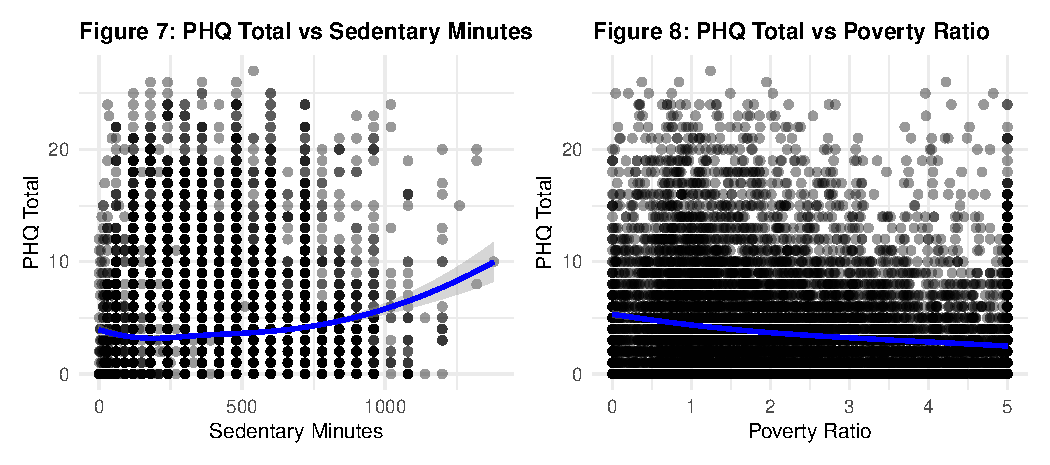
\includegraphics{report_files/figure-latex/plot_sedentary_poverty-1.pdf}

We also examined the relationship between PHQ scores and household size. The boxplot of integer variable \passthrough{\lstinline!hh\_size!} suggests that PHQ scores are relatively consistent across different household sizes. Given the lack of strong patterns in both cases and we do not consider them in model, this plots are not included in the main report but are available in the supplementary materials.

\subsection{Variable Description}\label{variable-description}

\textbf{Following are the variables left after the EDA:}

\textbf{Dependent variable (outcome):}

\begin{itemize}
\tightlist
\item
  \textbf{PHQ\_total}: Total score of the Patient Health Questionnaire-9 (PHQ-9), measuring depressive symptoms (range: 0--27).
\end{itemize}

\textbf{Independent variables (predictors):}

\emph{The following variables are categorical:}

\begin{itemize}
\tightlist
\item
  \textbf{gender}: Biological sex of the participant (Male or Female).
\item
  \textbf{race}: Self-identified race/ethnicity, categorized as Non-Hispanic White (reference), Non-Hispanic Black, Mexican American, Other Hispanic, Non-Hispanic Asian, or Other Race including Multi-Racial.
\item
  \textbf{birth\_country}: Country of birth: ``US-born'' or ``Foreign-born'' (reference: US-born).
\item
  \textbf{heavy\_drinker}: Whether consumed 4/5 or more alcoholic drinks per day in the past year (reference: No).
\item
  \textbf{diabetes}: Doctor-diagnosed diabetes status (reference: No).
\item
  \textbf{has\_asthma}: History of asthma diagnosis (reference: No).
\item
  \textbf{has\_liver}: History of liver condition (reference: No).
\end{itemize}

\emph{The following variables are numerical:}

\begin{itemize}
\tightlist
\item
  \textbf{sedentary\_minutes}: Minutes spent in sedentary activities on a typical day.
\item
  \textbf{poverty\_ratio}: Ratio of family income to poverty level (higher poverty ratios indicates higher income relative to the poverty threshold).
\item
  \textbf{age}: Participant age at time of interview.
\end{itemize}

\section{Model building}\label{model-building}

In this task, we aim to model the relationship between depressive symptoms and a set of demographic, behavioral, and health-related predictors. The goal is to identify significant associations and estimate the expected depression score given participants' characteristics.

The dependent variable \passthrough{\lstinline!PHQ\_total!} is a discrete, non-negative integer (ranging from 0 to 27) and most independent variables are either categorical or discrete numerical. Therefore, we consider discrete regression models, such as Poisson and Negative Binomial regression, to be appropriate starting points.

We initially fit a Poisson regression model. However, the model showed poor performance: it gave a high AIC and a Pearson dispersion statistic of 4.83, indicating substantial overdispersion in the data. This against the Poisson assumption that the mean and variance are equal, and suggests that the Poisson model is not suitable for this dataset.

\begin{align*}
Y_i &\sim \text{Poisson}(\mu_i) \\
\log(\mu_i) &= \beta_0 + \beta_1 \cdot \text{gender}_i + \beta_2 \cdot \text{race}_i + \beta_3 \cdot \text{birth\_country}_i \\
&\quad + \beta_4 \cdot \text{heavy\_drinker}_i + \beta_5 \cdot \text{diabetes}_i + \beta_6 \cdot \text{has\_asthma}_i \\
&\quad + \beta_7 \cdot \text{has\_liver}_i + \beta_8 \cdot \text{sedentary\_minutes}_i + \beta_9 \cdot \text{poverty\_ratio}_i+ \beta_10 \cdot \text{age}_i
\end{align*}

Due to the presence of overdispersion, both the quasi-Poisson and negative binomial models were considered. The quasi-Poisson model adjusts for overdispersion by scaling the standard errors so it does not support likelihood-based inference and cannot be used for formal model comparison. In contrast, the negative binomial model explicitly accounts for overdispersion and provides a valid likelihood framework, allowing for the use of information criteria such as AIC. Therefore, the negative binomial model was selected for further analysis. It can be seen that the AIC reduced significantly in negative binomial models compared to the Possion model.

\begin{align*}
Y_i &\sim \text{NegBin}(\mu_i, \theta) \\
\log(\mu_i) &= \beta_0 + \beta_1 \cdot \text{gender}_i + \beta_2 \cdot \text{race}_i + \beta_3 \cdot \text{birth\_country}_i \\
&\quad + \beta_4 \cdot \text{heavy\_drinker}_i + \beta_5 \cdot \text{diabetes}_i + \beta_6 \cdot \text{has\_asthma}_i \\
&\quad + \beta_7 \cdot \text{has\_liver}_i + \beta_8 \cdot \text{sedentary\_minutes}_i + \beta_9 \cdot \text{poverty\_ratio}_i+ \beta_10 \cdot \text{age}_i
\end{align*}

\begin{table}[!h]
\centering
\caption{\label{tab:NegBin}AIC Comparison between Poisson and Negative Binomial Models}
\centering
\resizebox{\ifdim\width>\linewidth\linewidth\else\width\fi}{!}{
\begin{tabular}[t]{l|l|l}
\hline
Model & df & AIC\\
\hline
Poisson model & 17 & 95357.47\\
\hline
Negative Binomial model & 18 & 68228.51\\
\hline
\end{tabular}}
\end{table}

To assess the contribution of individual predictors to the model, we examine the column \(\Pr\left(|z| > z_{\text{obs}}\right)\) in the regression output. This value represents the p-value for the null hypothesis that a given coefficient equals zero. A lower p-value indicates stronger evidence against the null hypothesis and suggests that the variable is statistically significant.

In this model, several levels of the categorical variables \passthrough{\lstinline!race!}, \passthrough{\lstinline!heavy\_drinker!}, and \passthrough{\lstinline!diabetes!} shows relatively high p-values.This suggest that they may not significantly improve model fit. To evaluate the overall contribution of these variables, we fitted three sub models by excluding each variable separately, and compared their AIC values to the original full model. As shown in the table, the full model (model\_nb) achieved the lowest AIC (68228.51), while all reduced model exhibited higher AICs. Therefore, we kept all three variable groups in the final model based on overall model fit, even though some individual coefficients within these variables were not statistically significant.

\begin{table}[!h]
\centering
\caption{\label{tab:NegBinSuM}Summary of Negative Binomial Regression Coefficients}
\centering
\resizebox{\ifdim\width>\linewidth\linewidth\else\width\fi}{!}{
\begin{tabular}[t]{l|l|l|l|l|l}
\hline
term & estimate & std.error & statistic & p.value & sig\\
\hline
(Intercept) & 1.7566 & 0.0472 & 37.2003 & < 2.2e-16 & \\
\hline
genderMale & -0.3264 & 0.0212 & -15.3832 & < 2.2e-16 & \\
\hline
raceMexican American & -0.1175 & 0.0381 & -3.0819 & 0.002057 & **\\
\hline
raceNon-Hispanic Asian & -0.2566 & 0.0472 & -5.4325 & 5.556e-08 & ***\\
\hline
raceNon-Hispanic Black & -0.1865 & 0.0292 & -6.3773 & 1.803e-10 & ***\\
\hline
raceOther Hispanic & 0.0578 & 0.0407 & 1.4188 & 0.155961 & \\
\hline
raceOther & 0.0739 & 0.0475 & 1.5551 & 0.119930 & \\
\hline
birth\_countryForeign-born & -0.1338 & 0.0326 & -4.1081 & 3.989e-05 & ***\\
\hline
heavy\_drinkerYes & 0.4398 & 0.0290 & 15.1597 & < 2.2e-16 & \\
\hline
heavy\_drinkerNA & -0.0997 & 0.0335 & -2.9763 & 0.002917 & **\\
\hline
diabetesYes & 0.2723 & 0.0303 & 8.9950 & < 2.2e-16 & \\
\hline
diabetesNA & 0.1779 & 0.0607 & 2.9311 & 0.003377 & **\\
\hline
has\_asthmaYes & 0.2597 & 0.0276 & 9.4153 & < 2.2e-16 & \\
\hline
has\_liverYes & 0.3423 & 0.0447 & 7.6631 & 1.814e-14 & ***\\
\hline
sedentary\_minutes & 0.0004 & 0.0001 & 8.6101 & < 2.2e-16 & \\
\hline
poverty\_ratio & -0.1298 & 0.0071 & -18.2335 & < 2.2e-16 & \\
\hline
age & -0.0060 & 0.0006 & -9.5125 & < 2.2e-16 & \\
\hline
\end{tabular}}
\end{table}

\begin{table}[!h][!h]
\centering\centering
\caption{\label{tab:subCompare}Negative Binomial Models Comparesion}
\centering
\resizebox{\ifdim\width>\linewidth\linewidth\else\width\fi}{!}{
\resizebox{\ifdim\width>\linewidth\linewidth\else\width\fi}{!}{
\begin{tabular}[t]{l|r|r}
\hline
Model & df & AIC\\
\hline
model\_nb & 18 & 68228.51\\
\hline
model\_nb\_race & 13 & 68311.30\\
\hline
model\_nb\_heavy\_drink & 16 & 68492.71\\
\hline
model\_nb\_diabetes & 16 & 68311.82\\
\hline
\end{tabular}}}
\end{table}
\newpage

\section{Model Refinement with Interactions}\label{model-refinement-with-interactions}

\subsection{Interaction visualization}\label{interaction-visualization}

To further improve the model and capture potential effect, we explored plausible interaction terms between key demographic and behavioral variables. Specifically, we generate relative plots to visually assess whether the association between individual predictors and depressive symptoms differs across relevant subgroups.

The interaction plots below suggest that gender moderates the effects of both sedentary time and age on depressive symptoms. Specifically, PHQ scores increase with sedentary minutes for both males and females, but the rise is sharper for females. Similarly, while depression scores decline with age in both sexes, females consistently report higher levels, and the decline is steeper in males with more waves. These patterns indicate that the effects of sedentary behavior and age on depression may vary by gender.

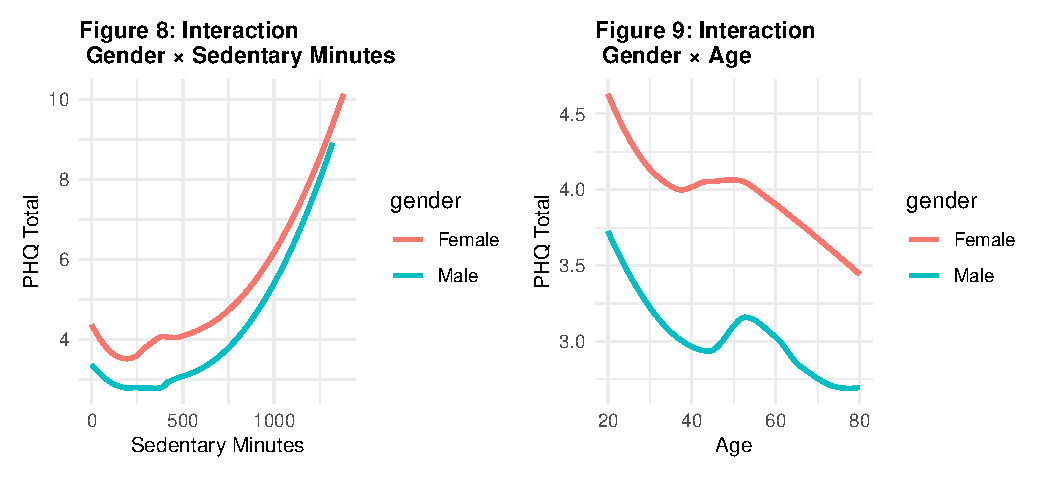
\includegraphics{report_files/figure-latex/interaction-1.pdf}

In contrast, the interaction between asthma status and age presents a different pattern. Individuals with asthma seem to have increasing depressive symptoms until middle age, followed by a decline. Whereas those without asthma show a more consistent decrease in depression across age. This suggests that asthma may amplify age-related differences in depressive symptoms.

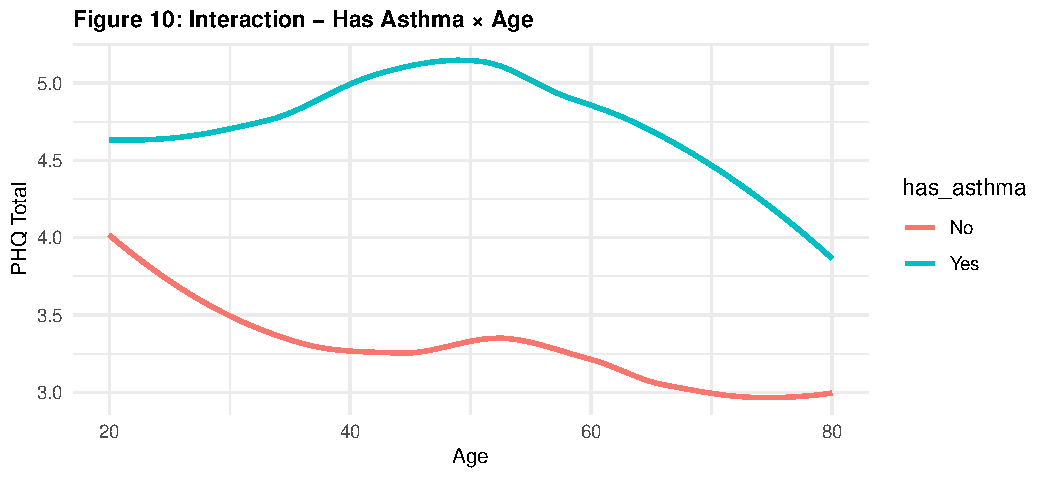
\includegraphics{report_files/figure-latex/interaction2-1.pdf}

\subsection{Model with interaction}\label{model-with-interaction}

According to these findings, we proceed to formally include the identified interaction terms in the regression model. Specifically, we include three interaction terms: \(gender \times sedentary\_minutes\), \(gender \times age\), and \(has\_asthma \times age\). These interactions are added to the full Negative Binomial model to capture potential effect modification and improve model fit.

The resulting model is expressed as:

\begin{align*}
Y_i &\sim \text{NegBin}(\mu_i, \theta) \\
\log(\mu_i) &= \beta_0 
+ \beta_1 \cdot \text{gender}_i 
+ \beta_2 \cdot \text{race}_i 
+ \beta_3 \cdot \text{birth\_country}_i 
+ \beta_4 \cdot \text{heavy\_drinker}_i \\
&\quad + \beta_5 \cdot \text{diabetes}_i 
+ \beta_6 \cdot \text{has\_asthma}_i 
+ \beta_7 \cdot \text{has\_liver}_i 
+ \beta_8 \cdot \text{sedentary\_minutes}_i \\
&\quad + \beta_9 \cdot \text{poverty\_ratio}_i 
+ \beta_{10} \cdot \text{age}_i 
+ \beta_{11} \cdot \text{gender}_i \cdot \text{sedentary\_minutes}_i \\
&\quad + \beta_{12} \cdot \text{gender}_i \cdot \text{age}_i
+ \beta_{13} \cdot \text{has\_asthma}_i \cdot \text{age}_i
\end{align*}

To assess the impact of interaction terms on model performance, we first fitted a full Negative Binomial model (\passthrough{\lstinline!model\_nb\_interact3!}) including all three interactions: \(gender \times sedentary\_minutes\), \(gender \times age\), and \(has\_asthma \times age\). However, the first and third interactions showed high p-values (\(\Pr(|z| > z_{\text{obs}})\)), indicating limited statistical significance. We therefore fitted a reduced model (\passthrough{\lstinline!model\_nb\_interact1!}) retaining only the \(gender \times age\) interaction. AIC comparisons showed that this simpler model achieved the lowest AIC, suggesting improved fit with fewer parameters. As a result, we chose to retain only the \(gender \times age\) interaction in the final model.

\begin{table}[!h]
\centering
\caption{\label{tab:table4}Negative Binomial Models Comparison with Interaction Terms}
\centering
\resizebox{\ifdim\width>\linewidth\linewidth\else\width\fi}{!}{
\begin{tabular}[t]{l|l|l}
\hline
Model & df & AIC\\
\hline
Full model & 18 & 68228.51\\
\hline
Model with all three interactions & 21 & 68225.83\\
\hline
Model with one interactions (gender * age) & 19 & 68224.95\\
\hline
\end{tabular}}
\end{table}

Now the model becomes:
\begin{align*}
Y_i &\sim \text{NegBin}(\mu_i, \theta) \\
\log(\mu_i) &= \beta_0 
+ \beta_1 \cdot \text{gender}_i 
+ \beta_2 \cdot \text{race}_i 
+ \beta_3 \cdot \text{birth\_country}_i 
+ \beta_4 \cdot \text{heavy\_drinker}_i \\
&\quad + \beta_5 \cdot \text{diabetes}_i 
+ \beta_6 \cdot \text{has\_asthma}_i 
+ \beta_7 \cdot \text{has\_liver}_i 
+ \beta_8 \cdot \text{sedentary\_minutes}_i \\
&\quad + \beta_9 \cdot \text{poverty\_ratio}_i 
+ \beta_{10} \cdot \text{age}_i 
+ \beta_{11} \cdot \text{gender}_i \cdot \text{age}_i
\end{align*}

\section{Model Diagnostics}\label{model-diagnostics}

\subsection{Goodness of fit}\label{goodness-of-fit}

To assess overall model fit, we evaluated the fit of the final Negative Binomial model using residual deviance, AIC, and log-likelihood. The model also achieved the lowest AIC (68,224.95) among all candidate models considered, reflecting an optimal balance between explanatory power and model complexity. Additionally, the log-likelihood (--34,093.47) further ensusing the model's adequacy in capturing the observed variation in depressive symptom scores.

\newpage

\begin{table}[!h]
\centering
\caption{\label{tab:goodfit}Model Fit Statistics for Negative Binomial Regression}
\centering
\resizebox{\ifdim\width>\linewidth\linewidth\else\width\fi}{!}{
\begin{tabular}[t]{l|r}
\hline
Metric & Value\\
\hline
Residual Deviance & 16337.3300\\
\hline
Degrees of Freedom & 14727.0000\\
\hline
Deviance / DF & 1.1093\\
\hline
AIC & 68224.9500\\
\hline
Log-Likelihood & -34093.4700\\
\hline
\end{tabular}}
\end{table}

\subsection{Residual Diagnostics}\label{residual-diagnostics}

Figure below shows diagnostic plots used to assess the model's residual behavior and potential influential observations. The Pearson residuals appear randomly scattered around zero, suggesting no major patterns or violations of model assumptions.

The fitted vs.~observed plot shows that the model generally captures the increasing trend in depressive symptom scores, but with substantial variability. While many points cluster around the diagonal line at lower fitted values, the spread increases as PHQ scores raise, which is typical for overdispersed count data (might caused by fewer participants report severe symptoms). This suggests that the model performs reasonably well in aggregate but has limited precision for individual predictions, especially at the upper range of the outcome.

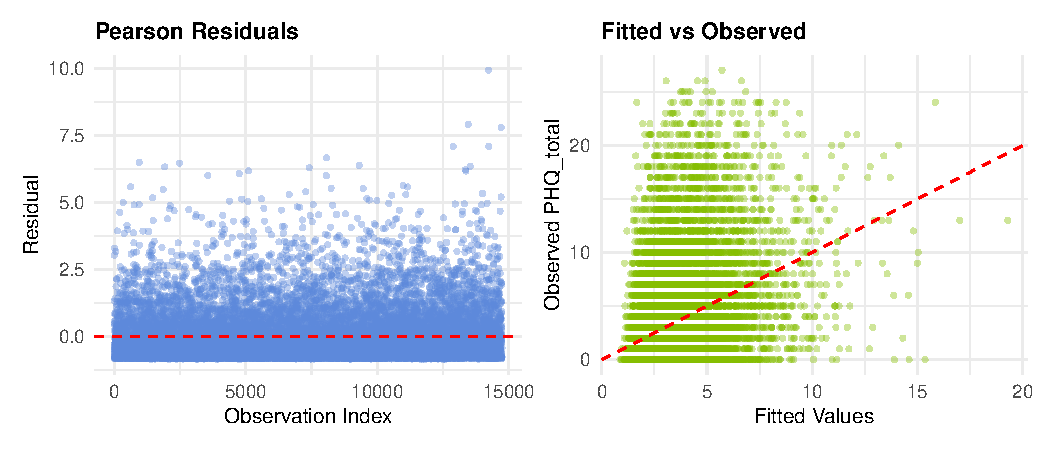
\includegraphics{report_files/figure-latex/Residuals1-1.pdf}
The QQ plot shows moderate deviation from the reference line, especially in the tails, suggesting some departure from the assumed residual distribution. However, for count data, this level of deviation is generally acceptable.

The Cook's distance plot shows that most observations have very low influence on the model. A small number of points lie above the common threshold, suggesting they may have mild influence, but none appear extreme. Overall, no strong outliers dominate the model fit.

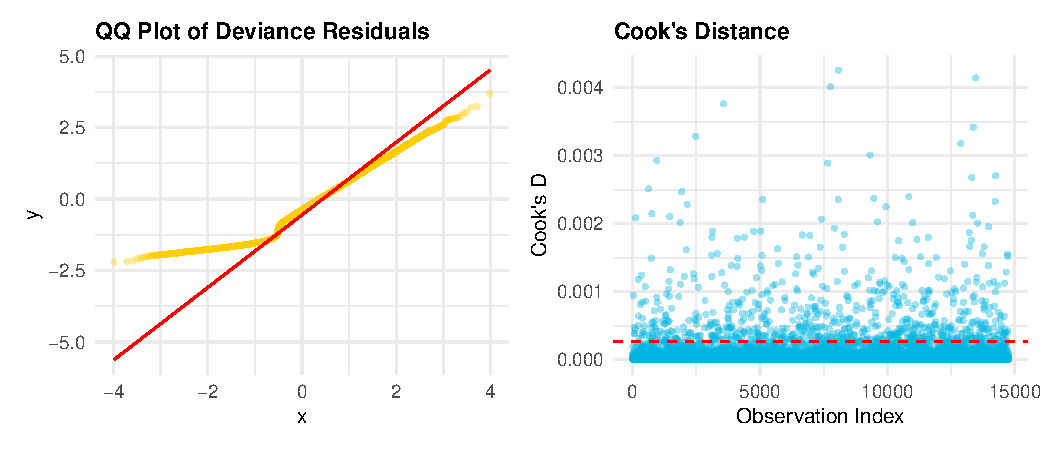
\includegraphics{report_files/figure-latex/Residuals2-1.pdf}

\section{Model Interpretation via IRR}\label{model-interpretation-via-irr}

To interpret the fitted negative binomial regression model, we exponentiate the estimated regression coefficients to obtain the Incidence Rate Ratios (IRRs). The IRR represents the multiplicative effect of a one-unit increase in a predictor on the expected count of the outcome variable (PHQ-9 total score), holding all other variables constant. For each predictor, a 95\% confidence interval is also calculated by \(\text{CI}_{95\%} = \exp\left( \hat{\beta} \pm 1.96 \cdot \text{SE} \right)\), indicating the range within which the true IRR is likely to fall. If this interval does not include 1, the predictor is considered statistically significant, meaning it has a meaningful association with the outcome. In the following section, we interpret the IRRs for each variable in the model to understand their effect on depression severity.

\begin{lstlisting}
##                                           IRR CI_lower CI_upper
## (Intercept)                             5.432    4.884    6.045
## sedentary_minutes                       1.000    1.000    1.001
## genderMale                              0.832    0.734    0.943
## age                                     0.995    0.994    0.997
## has_asthmaYes                           1.295    1.227    1.367
## raceMexican American                    0.888    0.824    0.957
## raceNon-Hispanic Asian                  0.773    0.705    0.849
## raceNon-Hispanic Black                  0.830    0.784    0.879
## raceOther Hispanic                      1.058    0.977    1.147
## raceOther Race - Including Multi-Racial 1.076    0.981    1.182
## birth_countryForeign-born               0.874    0.820    0.932
## heavy_drinkerYes                        1.555    1.469    1.646
## heavy_drinkerNA                         0.902    0.844    0.963
## diabetesYes                             1.317    1.241    1.397
## diabetesNA                              1.196    1.064    1.349
## has_liverYes                            1.410    1.293    1.540
## poverty_ratio                           0.878    0.866    0.890
## genderMale:age                          0.997    0.995    1.000
\end{lstlisting}

\textbf{(Intercept)}: When all predictors are at their reference level or zero, the expected count of the PHQ-9 score is 5.432 times higher than the baseline (which is 1 under the log-link function).

\textbf{sedentary\_minutes}: For each additional minute of sedentary time, the expected PHQ-9 score increases only slightly. However, this may still be meaningful in aggregate, as the variable's scale is large.

\textbf{genderMale}:Males have an expected PHQ-9 score that is 17\% lower than females on average. This effect is statistically significant.

\textbf{age}: For each 1 year increase in age, the expected PHQ-9 score decreases by 0.5\%, holding all else constant

\textbf{has\_asthmaYes}: Participants with asthma have PHQ-9 scores that are 29.5\% higher than those without asthma. This is statistically significant.

\textbf{raceMexican American}: Mexican American individuals are expected to have PHQ-9 scores that are 11.2\% lower than Non-Hispanic White individuals, holding all else constant. This is statistically significant.

\textbf{raceNon-Hispanic Asian}: Non-Hispanic Asian participants have PHQ-9 scores that are 22.7\% lower than Non-Hispanic Whites. There is strong evidence of significantly lower depression scores in this group.

\textbf{raceNon-Hispanic Black}: Non-Hispanic Black individuals have PHQ-9 scores that are 17.0\% lower than Non-Hispanic Whites. This is statistically significant.

\textbf{raceOther Hispanic}: Other Hispanic participants have PHQ-9 scores that are 5.8\% higher than Non-Hispanic Whites. This is not statistically significant.

\textbf{raceOther Race - Including Multi-Racial}: This group shows PHQ-9 scores that are 7.6\% higher than Non-Hispanic Whites. This is not statistically significant.

\textbf{birth\_countryForeign-born}: Participants born outside the U.S. have PHQ-9 scores that are 12.6\% lower than U.S.-born individuals, adjusting for other variables. This effect is statistically significant.

\textbf{heavy\_drinkerYes}: Heavy drinkers have PHQ-9 scores that are 55.5\% higher than non-heavy drinkers. This is a strong and statistically significant effect.

\textbf{heavy\_drinkerNA}: Participants with missing alcohol data have PHQ-9 scores that are 9.8\% lower than the reference group. This is statistically significant. The missing values for variables such as diabetes status might be caused by a lack of medical knowledge or absence of formal diagnosis. While questions about alcohol consumption are typically within personal awareness. Therefore, refusal or omission in this case may represent a deliberate choice rather than ignorance, potentially reflecting discomfort and denial bias.

\textbf{diabetesYes}: People with diabetes have PHQ-9 scores that are 31.7\% higher than those without diabetes. There is a strong and significant association.

\textbf{diabetesNA}: Participants with missing diabetes status have PHQ-9 scores that are 19.6\% higher than the reference group. Unlike the alcohol variable, the missing value here may reflect a lack of knowledge rather than participant choice.

\textbf{has\_liverYes}: Participants reporting liver conditions have PHQ-9 scores that are 41\% higher than those without. This is statistically significant.

\textbf{poverty\_ratio}: For every unit increase in poverty ratio (i.e., higher income relative to the poverty line), PHQ-9 scores decrease by approximately 12.2\%. This suggests that higher socioeconomic status is strongly protective against depressive symptoms.

\textbf{genderMale:age}: This interaction indicates that as age increases, the difference in depression between males and females narrows slightly. Specifically, each additional year reduces the male--female difference by about 0.3\%. This effect is not statistically significant.

\section{Limitations and Next Steps}\label{limitations-and-next-steps}

This analysis has several limitations that should be acknowledged. First, due to the limited number of common variables across NHANES cycles and a high rate of item non-response, the usable sample size was reduced. This highly affects the statistical power and generalizability. We could consider including more relevant variables from other NHANES modules (e.g., dietary, physical exam, blood data). We can also consider imputation techniques to handle missing data more robustly.

Second, extending the study period (e.g., 2005--2020) could improve sample size and representativeness. However, this might result in fewer common variables across years. We need careful trade-offs between these aspects.

Third, we observed overdispersion in the PHQ-9 score distribution and a strong concentration of values between 0 and 3. This highly influences the accuracy of the developed model. One possible solution is to stratify the population into binary or ordinal outcome groups and apply logistic or ordinal regression. Alternatively, we can also trim or exclude the participants with very low PHQ scores and focus on modeling moderate to severe symptoms. This can yield more stable estimates of associated risk factors.

As a follow-up, we re-fitted the model after excluding data with PHQ-9 scores lower than 4. Without the large noise from floor effects, the estimates for most predictors became more stable and interpretable. Additionally, the model's AIC was significantly reduced, suggesting improved overall fit. However, the reduced sample size may limit statistical power and increase uncertainty in the estimates. Future work could further explore stratified modeling or appropriate thresholding methods while ensuring adequate sample representation

\begin{table}[!h]
\centering
\caption{\label{tab:phqdata3}Model Fit Summary for Subset (PHQ > 3)}
\centering
\begin{tabular}[t]{l|r}
\hline
Metric & Value\\
\hline
AIC & 27844.70\\
\hline
Residual Deviance & 4828.90\\
\hline
Null Deviance & 5174.29\\
\hline
Deviance / DF & 0.95\\
\hline
\end{tabular}
\end{table}

Fourth, many of the identified covariates may only affect moderate to severe depression. This lack of effect in the lower PHQ range may dilute the observed associations when using a single regression model across all PHQ levels.

Lastly, because the primary goal of this analysis was explanatory rather than predictive, we did not split the dataset into training and testing sets. Instead, we relied on model diagnostics (e.g., residual plots, AIC, dispersion statistics) to assess fit and guide model selection. However, future studies focused on prediction should evaluate generalizability using cross-validation or holdout testing.

\section{References}\label{references}

\end{document}
